% Merged manuscript: LIC-RQ-v2 (Study 1) + CDR-Stream (Study 2).
% Claim boundaries: MERGED_PAPER_CLAIMS.md (approved 2026-10-04) -- binding.
% Numbers: generated/numbers.tex (Study 1, scripts/paper_lic_rq_v2_assets.py --paper paper/merged)
%          generated/cdr_numbers.tex (Study 2 + cross-study, scripts/paper_merged_cdr_assets.py)
% Cross-references to the supplement (supp-...) need supplement.aux:
% compile supplement.tex first, then main.tex.
\documentclass[preprint,11pt,authoryear]{elsarticle}

\usepackage[T1]{fontenc}
\usepackage[utf8]{inputenc}
\usepackage{amsmath,amssymb}
\usepackage{booktabs,array}
\usepackage{graphicx}
\usepackage{xcolor}
\usepackage{tikz}
\usetikzlibrary{positioning,arrows.meta}
\usepackage{xr}
\externaldocument[supp-]{supplement}
\usepackage[hidelinks]{hyperref}

\renewcommand{\bibfont}{\small}
\setlength{\bibsep}{1.5pt plus 0.5pt}
\graphicspath{{figures/}}
% Generated by scripts/paper_lic_rq_v2_assets.py
\newcommand{\nRecords}{11{,}382}
\newcommand{\nTasks}{48}
\newcommand{\nEmptyPrimaries}{6}
\newcommand{\nPermutations}{10{,}000}
\newcommand{\recordsSha}{e313f1ce5985}
\newcommand{\Ktemp}{0.7}
\newcommand{\Krep}{5}
\newcommand{\Lpar}{2}
\newcommand{\maxTok}{2{,}048}
\newcommand{\dialGpt}{0.688}
\newcommand{\freshGpt}{0.896}
\newcommand{\diffGpt}{0.208}
\newcommand{\ciGpt}{[0.063, 0.354]}
\newcommand{\pHolmGpt}{0.026}
\newcommand{\pRawGpt}{0.013}
\newcommand{\dialLlama}{0.854}
\newcommand{\freshLlama}{0.958}
\newcommand{\diffLlama}{0.104}
\newcommand{\ciLlama}{[0.000, 0.208]}
\newcommand{\pHolmLlama}{0.125}
\newcommand{\pRawLlama}{0.125}
\newcommand{\dialMistral}{0.063}
\newcommand{\freshMistral}{0.354}
\newcommand{\diffMistral}{0.292}
\newcommand{\ciMistral}{[0.146, 0.438]}
\newcommand{\pHolmMistral}{0.004}
\newcommand{\pRawMistral}{0.001}
\newcommand{\nFreshOnly}{34}
\newcommand{\nDialOnly}{5}
\newcommand{\crlAuroc}{0.627}
\newcommand{\crlCi}{[0.493, 0.760]}
\newcommand{\crlP}{0.022}
\newcommand{\crlPairs}{687}
\newcommand{\robAllAuroc}{0.571}
\newcommand{\robAllP}{0.057}
\newcommand{\robAllCi}{[0.484, 0.656]}
\newcommand{\robExclAuroc}{0.569}
\newcommand{\robExclP}{0.059}
\newcommand{\robExclCi}{[0.483, 0.655]}
\newcommand{\replayCandidates}{0}
\newcommand{\replaySensCandidates}{0}

% Generated by scripts/paper_merged_cdr_assets.py
\newcommand{\cdrGptEarly}{0.61}
\newcommand{\cdrGptLate}{0.09}
\newcommand{\cdrGptCtrlLate}{0.64}
\newcommand{\cdrLevelMatched}{-0.118}
\newcommand{\cdrLevelMatchedP}{$<$0.001}
\newcommand{\cdrLevelMatchedN}{90}
\newcommand{\cdrLevelMatchedSzeroE}{-0.185}
\newcommand{\ctrlScreenDetect}{0/18}
\newcommand{\earlyCqSignal}{18/18}
\newcommand{\earlyCqNull}{3/12}
\newcommand{\earlyLsSignal}{10/18}
\newcommand{\earlyLsNull}{4/12}
\newcommand{\earlyLsBefore}{7}
\newcommand{\replaySsDeltaGpt}{+0.46}
\newcommand{\replaySsDeltaLlama}{+0.42}
\newcommand{\replayLsDeltaGpt}{+0.31}
\newcommand{\crlLastGapAuroc}{0.672}
\newcommand{\crlLastGapP}{0.001}
\newcommand{\crlCondAuroc}{0.468}
\newcommand{\crlCondP}{0.674}


% Primitive input inside tabular (LaTeX's \input is not safe before \bottomrule).
\makeatletter
\newcommand{\inputtable}[1]{\@@input #1 }
\makeatother

\journal{Expert Systems with Applications}

\begin{document}

\begin{frontmatter}

\title{The Silent Cost of Conversation History in LLM Reasoning}

\author[tarsus]{Ali \c{S}enol\corref{cor1}}
\ead{alisenol@tarsus.edu.tr}
\cortext[cor1]{Corresponding author.}
\affiliation[tarsus]{organization={Tarsus University},
  city={Tarsus, Mersin}, country={T\"urkiye}}

\begin{abstract}
Large language models (LLMs) are increasingly used in multi-turn settings in
which a task unfolds over many exchanges. Their own earlier replies and an
accumulating task state become part of the context they reason from. We ask
whether this degrades reasoning success, and whether the degradation can be
detected early from measures of reasoning quality.

We combine two complementary, prospectively frozen studies. Study~1 uses short,
sharded math tasks from the Lost in Conversation benchmark. Each of three models
answers every turn twice with identical user information, with and without its
own prior replies. Study~2 is a purpose-built, 100-turn benchmark with exact
per-turn answers, calibrated difficulty and scheduled difficulty shifts. Its
dialogues are answered either from the full dialogue history or from a verified
state summary.

Retaining assistant replies lowered final success in Study~1, significantly for
two of three models. In Study~2, accuracy under full history fell sharply within
about twenty turns, even when difficulty was held fixed. A verified state
summary preserved accuracy in all three models. Neither the
reasoning-quality metrics we examined nor a paired process measure warned of
these failures in a robust, model-general way. Coherence and stability even
rose as accuracy fell.

Long interactions can therefore degrade LLM reasoning in ways that single-stream
quality monitoring does not reveal. Compact, verified state representations are
a promising mitigation.

\end{abstract}

\begin{keyword}
large language models \sep multi-turn dialogue \sep conversation history \sep
state tracking \sep reasoning quality \sep drift detection \sep early warning
\end{keyword}

\end{frontmatter}

\section{Introduction}
\label{sec:introduction}

Large language models (LLMs) are moving from single-question assistants to
components of expert and decision-support systems that keep a task alive over
many turns. A procurement assistant tracks a budget as invoices arrive, a
logistics assistant follows stock across warehouses, and a laboratory assistant
records volumes as reagents are transferred. In each case the user supplies
information piece by piece, corrects earlier statements and asks questions
whose answers depend on everything said so far. The model's context therefore
accumulates two things: its own earlier replies and a task state that changes
at every turn. We call this accumulated context the \emph{conversation
history}. In our experiments, the condition that retains it is called
\emph{dialogue history}.

There is growing evidence that this setting is costly.
\citet{laban2025lost} showed that performance drops substantially when the
information of a single-turn task is revealed over several turns: models commit
to early answers and fail to recover. \citet{huang2026benefit} showed that
removing the assistant's own previous replies often preserves or improves
response quality, a harm they call \emph{context pollution}. Long-context
benchmarks show that information in long contexts is not used uniformly
\citep{liu2024lost}, while prior assistant errors can propagate through later
turns \citep{huang2026benefit}.

For a system designer, two operational questions follow, and prior work does
not settle either of them. The first is whether degradation persists, or
accelerates, over long horizons once task difficulty is controlled. Long
dialogues naturally change what they ask, so a falling accuracy curve may
reflect harder questions rather than a harder context. The second is whether
the degradation can be detected \emph{before} accuracy fails. A deployed system
rarely observes the correct answer, so it must rely on observable process
signals. Reasoning quality has been decomposed into dimensions such as
agreement between samples, robustness to rewording, logical coherence of the
reasoning chain and stability of the trace \citep{rqeval2026}. If these
dimensions deteriorated before accuracy, they could serve as an early-warning
layer, and classic drift detectors could turn them into alarms with controlled
false-alarm rates \citep{gama2014survey,lu2019learning}. ERGO uses token-entropy
spikes in a related role \citep{khalid2025ergo}. To our knowledge, whether
established process metrics warn under accumulated history has not been tested
under prospectively fixed analyses with calibrated false alarms.

We address both questions with two complementary studies. Each was analysed
under a protocol frozen before its data were collected, and every analysis
added later is labelled as exploratory or post-hoc.
\emph{Study~1} uses the math tasks of Lost in Conversation
\citep{laban2025lost}. At every turn, each model answers twice from identical
user information, once with and once without its own earlier replies, which
yields a task-paired estimate of the net effect of retaining assistant-side
history. \emph{Study~2} introduces CDR-Stream, a purpose-built benchmark of
100-turn state-tracking dialogues with exact per-turn answers, difficulty
calibrated separately for each model, and scheduled difficulty shifts. Its
control arm replaces the history with a solver-verified state summary. Across
both studies we then test the measurable quality metrics, a paired readiness
measure and window-based drift detectors as early-warning signals. The two
studies use different tasks, models and controls. We therefore read them as
revealing complementary failure modes, not as one dose--response curve.

The paper makes four contributions.
\begin{enumerate}
  \item A frozen, task-paired confirmatory estimate of the effect of retaining
    assistant replies on exactly scored multi-turn math tasks. It replicates
    the direction reported by \citet{huang2026benefit} under a prospectively
    fixed analysis; it is a replication, not a discovery.
  \item CDR-Stream, a long-horizon benchmark with exact per-turn gold and
    per-model difficulty calibration. In it, accuracy under full history
    collapsed within about twenty turns, even at matched difficulty, while a
    verified state summary preserved it in all three models tested.
  \item A prospective test of early warning. The measurable consistency,
    coherence and stability metrics did not predict failure. Coherence and
    stability even stayed level or rose as accuracy fell. A paired readiness
    measure reduced to the persistence of the current unresolved state, and
    single-stream detectors were too weak for the observed drifts.
  \item Design guidance for LLM-based expert systems, supported by a detector
    power simulation and a detector audit: manage state explicitly, monitor by
    comparison or aggregation across sessions, and verify that a baseline
    detector can fire on streams of the intended length.
\end{enumerate}

Section~\ref{sec:related} reviews related work and positions the monitoring
framework. Sections~\ref{sec:study1} and~\ref{sec:study2} present the studies,
their metrics and evidence standards, and
Section~\ref{sec:monitoring} asks whether the degradation can be detected
early. Section~\ref{sec:discussion} discusses implications and limitations.

\section{Related work}
\label{sec:related}

\paragraph{Multi-turn degradation.}
Several benchmarks evaluate conversational ability over multiple exchanges,
including MT-Bench \citep{zheng2023judging}, MT-Eval \citep{kwan2024mteval} and
MINT \citep{wang2024mint}.

\citet{laban2025lost} showed that LLMs lose substantial performance when a fully
specified instruction is sharded across turns, mainly through increased
unreliability. \citet{huang2026benefit} compared full conversational context with
contexts from which assistant turns are omitted or condensed, using in-the-wild
conversations and the Lost in Conversation math tasks. They found that response
quality is largely preserved under aggressive filtering, and that prior assistant
replies can propagate errors (context pollution).

Our Study 1 replicates this assistant-omission contrast with a frozen,
task-paired analysis. Study 2 extends the question to 100-turn dialogues with
exact answers and controlled difficulty.

Related single-turn failure modes include:
\begin{itemize}
  \item sensitivity to long inputs \citep{liu2024lost};
  \item distraction by irrelevant context \citep{shi2023distracted};
  \item unreliable self-correction \citep{huang2024cannot}.
\end{itemize}

\paragraph{Mitigation by context management.}
Two lines of work restructure the context to recover performance:
\begin{itemize}
  \item ERGO \citep{khalid2025ergo} detects entropy spikes and consolidates the
    prompt;
  \item \citet{huang2026benefit} filter assistant turns.
\end{itemize}
Our Study 2 control arm is a verified state summary. It belongs to this family,
but it uses solver-verified state, so it serves as an upper bound on what state
compression can achieve.

\paragraph{Reasoning-quality dimensions.}
Beyond final accuracy, reasoning quality has been characterized in several ways:
\begin{itemize}
  \item agreement across samples \citep{wang2023selfconsistency};
  \item faithfulness and coherence of chains of thought
    \citep{turpin2023say,lanham2023measuring};
  \item self-knowledge \citep{kadavath2022know}.
\end{itemize}
We use the six-dimension decomposition of RQEval \citep{rqeval2026}:
\begin{itemize}
  \item answer accuracy (CQ);
  \item consistency (CS);
  \item robustness (RS);
  \item logical coherence (LS), computed with an NLI model \citep{he2021deberta};
  \item efficiency (ES);
  \item stability (SS), computed with BERTScore \citep{zhang2020bertscore}.
\end{itemize}
We test whether these dimensions warn; we do not modify them.

\paragraph{Drift detection.}
Classic stream detectors include:
\begin{itemize}
  \item CUSUM \citep{page1954continuous};
  \item Page--Hinkley \citep{hinkley1971inference};
  \item EWMA charts \citep{roberts1959control};
  \item DDM \citep{gama2004learning};
  \item ADWIN \citep{bifet2007learning}.
\end{itemize}
Surveys of concept drift include \citet{gama2014survey} and
\citet{lu2019learning}. Shift detection for deployed models is studied by
\citet{rabanser2019failing}, and behavioural drift of commercial LLMs over time
by \citet{chen2024chatgpt}. We apply these detectors to per-turn
reasoning-quality streams under calibrated false-alarm control.

\paragraph{Prospective analysis plans.}
Model evaluations are prone to analytic flexibility in prompts, parsers and
thresholds. Fixing hypotheses and analyses in advance \citep{nosek2018preregistration}
limits it, so we froze each study's protocol before its data, and we label every
post-hoc analysis as such.

\section{Monitoring framework and evaluation design}
\label{sec:framework}

This section defines what both studies share: the context policies, the
per-turn quality signals, the streaming monitor and the evidence standards
(Figure~\ref{fig:framework}).

\begin{figure}[!htbp]
\centering
\begin{tikzpicture}[
  font=\small, >=Latex, node distance=4mm and 6mm,
  box/.style={draw, rounded corners=2pt, align=center, minimum height=9mm,
              inner sep=3pt, fill=#1},
  box/.default=white]
\node[box=gray!10, text width=27mm] (user) {User turn $u_t$\\(new information,\\question)};
\node[box=blue!8, text width=33mm, right=of user] (policy)
  {Context policy $\pi$\\[1pt]\footnotesize dialogue history $\cdot$ fresh prefix\\
   \footnotesize $\cdot$ verified state summary};
\node[box=gray!10, text width=24mm, right=of policy] (llm) {LLM\\primary reply\\+ $K{-}1$ samples\\+ $L$ rewordings};
\node[box=orange!10, text width=26mm, below=9mm of llm] (metrics)
  {Per-turn quality\\vector $\mathbf{q}_t$\\\footnotesize CQ CS RS LS ES SS};
\node[box=orange!10, text width=27mm, left=of metrics] (window)
  {Window means\\$\bar q_{m,t}$ over the last\\$W$ valid values};
\node[box=red!8, text width=30mm, left=of window] (detect)
  {Drift detectors\\\footnotesize CUSUM, PH, EWMA,\\\footnotesize DDM, ADWIN};
\node[box=green!10, text width=30mm, below=8mm of detect] (alarm)
  {Alarm time $\tau_m$\\\footnotesize compared with the change $c$};
\node[box=green!10, text width=27mm, right=of alarm] (null)
  {Threshold from\\stationary nulls\\\footnotesize false alarms $\le\alpha$};
\node[box=gray!5, text width=26mm, right=of null] (gold)
  {Exact gold $y_t$\\\footnotesize(evaluation only)};
\draw[->] (user) -- (policy);
\draw[->] (policy) -- (llm);
\draw[->] (llm) -- (metrics);
\draw[->] (metrics) -- (window);
\draw[->] (window) -- (detect);
\draw[->] (detect) -- (alarm);
\draw[->, dashed] (null) -- (alarm);
\draw[->, dashed] (gold) -- (null);
\draw[->, dashed] (gold.north) -- (metrics.south);
\draw[->, dotted] (llm.north) -- ++(0,4mm) -| node[pos=0.25, above, font=\footnotesize]
  {primary reply enters later history (dialogue history only)} (policy.north);
\end{tikzpicture}
\caption{The monitoring framework. A context policy decides what the model
sees at turn $t$. Responses are scored into a per-turn quality vector, smoothed
over a window and passed to drift detectors whose thresholds are calibrated on
stationary dialogues. Exact gold is used only to score accuracy and evaluate
alarms, never by the monitor.}
\label{fig:framework}
\end{figure}

\subsection{Context policies}

At turn $t$ the user sends $u_t$ and the model returns a primary reply $r_t$
from a context $C_t$ set by a policy $\pi$:
\begin{align}
  \text{dialogue history:}\quad & C_t = (u_1, r_1, \dots, r_{t-1}, u_t),\\
  \text{fresh prefix:}\quad & C_t = (u_1, \dots, u_t),\\
  \text{verified state summary:}\quad & C_t = (s_{t-1}, u_t),
\end{align}
where $s_{t-1}$ is the exact task state after turn $t-1$, rendered by a
solver. Dialogue history versus fresh prefix estimates the \emph{net} effect of
retaining assistant-side history; context length and message positions differ
as well, so the effect is not attributed to the content of the replies alone.
The verified state summary shortens the context, removes earlier replies and
supplies a correct state at once; it tests mitigation, not mechanism. Our code
packs every context into the request, with server-side memory, retrieval and
prompt rewriting disabled, after a pilot in which a gateway silently dropped
native message history. Every context is therefore reproducible from the
stored records.

\subsection{Per-turn quality signals}

Each primary reply is accompanied by $K-1$ further samples from the same
context and by $L$ replies to frozen rewordings of the instruction. RQEval
\citep{rqeval2026} computes six dimensions in $[0,1]$, used unchanged:
accuracy (CQ, the primary answer equals the gold); consistency (CS, pairwise
agreement of the $K$ answers); robustness (RS, agreement of reworded replies
with a correct primary answer); logical coherence (LS, absence of NLI
contradictions between consecutive steps; \citealp{he2021deberta}); efficiency
(ES, correctness combined with token economy); and stability (SS, BERTScore
similarity of the $K$ traces; \citealp{zhang2020bertscore}). CQ, RS and ES
require a final answer and gold, CS needs at least two answers, and LS and SS
need only reasoning text. This matters for early warning: a signal that
requires an answer is unobservable before the model is ready to give one.
Missing values are never imputed and are reported with their support.

\subsection{The streaming monitor}

For each metric $m$, the monitor keeps a trailing mean $\bar q_{m,t}$ over the
last $W\in\{10,20,30\}$ valid values ($W=20$ primary); missing values neither
enter nor advance the window. Five detectors, CUSUM, Page--Hinkley (PH), EWMA,
DDM and ADWIN, are paired with metrics by three strategies taken from the
funded project design (Table~\ref{tab:strategies}). Thresholds are never tuned
on drift data: for each metric, detector and window, we take the most
sensitive grid value whose first-alarm rate on stationary streams does not
exceed $\alpha$. Study~1 uses permutation nulls with family-wise
$\alpha=0.05$ verified on disjoint permutations. Study~2 uses its stationary
dialogues, with leave-one-out false-alarm estimates. For a change at turn $c$,
an alarm before $c$ is a false alarm and an alarm in $[c, c+33]$ a detection.
A signal gives \emph{early warning} only if it detects drifts in time, respects
the null calibration and does so across models.

\begin{table}[!htbp]
\centering
\caption{Detector assignment strategies. All monitor a decrease of the window
mean; CQ is additionally monitored on its raw binary stream by DDM.}
\label{tab:strategies}
\footnotesize
\setlength{\tabcolsep}{4pt}
\begin{tabular}{lcccccc}
\toprule
Strategy & CQ & CS & RS & LS & ES & SS\\
\midrule
Distribution-based & CUSUM & CUSUM & CUSUM & CUSUM & CUSUM & CUSUM\\
Proposal mapping & CUSUM & ADWIN & DDM & PH & EWMA & ADWIN\\
ADWIN everywhere & ADWIN & ADWIN & ADWIN & ADWIN & ADWIN & ADWIN\\
\bottomrule
\end{tabular}
\end{table}

\subsection{A paired readiness measure}

Sharded tasks allow an answer-free paired signal. Let $a_t^{\mathrm{F}}$ and
$a_t^{\mathrm{D}}$ be 1 if the fresh-prefix and dialogue-history arms attempt an
answer at turn $t$, and 0 if they state that more information is needed. The
\emph{Cumulative Resolution Lag} of a task is
\begin{equation}
  \mathrm{CRL} = \frac{1}{|\mathcal{T}|}\sum_{t\in\mathcal{T}}
  \max\!\left(a_t^{\mathrm{F}}-a_t^{\mathrm{D}},\,0\right),
\end{equation}
over the pre-final turns $\mathcal{T}$ at which both arms responded validly.
CRL measures how persistently the history arm lags an information-matched
counterfactual in becoming ready to answer. It was frozen as an auxiliary
measure before the Study~1 data were collected and is not an RQEval dimension.

\subsection{Evidence standards}

Every result carries one of four labels. \emph{Confirmatory} results test
hypotheses frozen before data collection; \emph{prespecified secondary}
results are frozen but outside the confirmatory family; \emph{exploratory}
results use rules fixed before computation on data already seen; and
\emph{post-hoc} results were designed after inspection. Protocols fixed the
sample, prompts, models, scoring, missing-data policy and tests, and were
hashed together with all input records. Raw responses are stored before scoring
and never overwritten, failed gates are reported rather than relabelled, and
every number, table and figure is regenerated by scripts from the hashed
inputs.

\section{Study 1: the paired effect of retaining assistant replies}
\label{sec:study1}

\subsection{Design}

\paragraph{Tasks and sample.}
We used the public math subset of Lost in Conversation \citep{laban2025lost}:
103 GSM8K-derived problems \citep{cobbe2021training}, each split into ordered
information shards, with one shard revealed per turn. Before any model was
queried, an input audit excluded 17 tasks. Eleven duplicated inputs of our
earlier experiments, eight appeared to change meaning when sharded, and two
belonged to both groups. A deterministic hash-based procedure that used no model
output then drew \nTasks{} science tasks with 4--9 shards (median 6) and four
disjoint integration tasks. The integration stage checked only transport,
resumption, parsing, scorers and plotting, and its outcomes could not alter the
sample or the analysis.

\paragraph{Models and arms.}
Three models were accessed through an academic gateway: GPT-4o-mini
\citep{openai2024gpt4o}, Llama-4 Scout and Mistral-7B \citep{jiang2023mistral}.
At every turn $t$, each model answered twice from identical user shards
$1,\dots,t$: in the dialogue-history arm, its own earlier primary replies were
interleaved; in the fresh-prefix arm, they were omitted
(Section~\ref{sec:framework}). The system prompt asked the model to solve
incrementally from the information given and stated that earlier assistant
replies might be wrong. Every reply had to end with exactly one line,
\texttt{FINAL\_ANSWER: <number>} once the answer was determined, or
\texttt{STATUS: NEED\_MORE\_INFORMATION} otherwise. Each cell received
$K=\Krep{}$ same-context samples and $L=\Lpar{}$ replies to frozen rewordings
of the instruction, at temperature \Ktemp{} and a \maxTok{}-token ceiling. Only
the primary sample entered later history.

The acquisition produced \nRecords{} successful calls, none truncated. Six
Mistral-7B primaries were empty despite a successful status. They were kept as
invalid, never retried, and represented in later history by a fixed
placeholder. Integration showed that the original strict final-line parser
rejected many replies that did contain an explicit marker. Before the science
run we therefore froze a parser that still requires the marker but tolerates
numbering, units and minor variants. Strict scores are preserved alongside.

\paragraph{Frozen analysis.}
The primary endpoint was paired final-turn success, tested by exact McNemar
tests \citep{mcnemar1947note} with task-bootstrap 95\% confidence intervals
(\nPermutations{} resamples; \citealp{efron1979bootstrap}) and Holm correction
across the three models \citep{holm1979simple}. Before the last shard, most
tasks have no determined answer, so CQ, RS and ES are structurally unobservable
there. The pre-final warning candidates were therefore CS, LS and SS. Each was
tested by a task-clustered partial correlation with final failure in the
dialogue arm, adjusting for model, turn, the revealed-information fraction and
log context length, with one-sided task-clustered permutation tests and Holm
correction across the three metrics. CRL was frozen as an auxiliary measure;
its target was a positive final readiness gap, in which the fresh prefix
attempts an answer while the history arm remains unresolved.

\subsection{Results}

\paragraph{Retaining assistant replies lowers final success (confirmatory).}
Table~\ref{tab:s1primary} and Figure~\ref{fig:s1} report the primary endpoint.
Final success fell from \freshGpt{} in the fresh prefix to \dialGpt{} under
dialogue history for GPT-4o-mini (difference \diffGpt{}, 95\% CI \ciGpt{},
Holm $p=\pHolmGpt$) and from \freshMistral{} to \dialMistral{} for Mistral-7B
(\diffMistral{}, CI \ciMistral{}, Holm $p=\pHolmMistral$). Llama-4 Scout
showed the same direction (\diffLlama{}, CI \ciLlama{}) without confirmatory
significance (Holm $p=\pHolmLlama$). Discordant tasks were strongly
asymmetric across models: in \nFreshOnly{} tasks only the fresh prefix
succeeded, in \nDialOnly{} only the history arm did. Restricting the analysis
to tasks whose final replies were format-valid in both arms left the GPT-4o-mini
and Mistral-7B effects intact (supplementary Table~S3).

The Mistral-7B case shows how such a harm can arise. With its own replies in
context, the model tended to remain in an explicit ``need more information''
state at the last turn. Given the same information without those replies, it
attempted an answer. The history did not merely add noise to the computation; it
changed whether the model regarded the task as solvable.

\begin{table}[t]
\centering
\caption{Study 1 paired final-turn success over \nTasks{} tasks per model.
F/D: number of tasks in which only the fresh prefix, or only the dialogue
history, succeeded. $p$: exact McNemar test.}
\label{tab:s1primary}
\small
\resizebox{\linewidth}{!}{%
\begin{tabular}{lcccccc}
\toprule
Model & Dialogue history & Fresh prefix & Diff.\ [95\% CI] & F/D & $p$ & $p_{\text{Holm}}$\\
\midrule
\inputtable{generated/table_primary.tex}
\bottomrule
\end{tabular}
}
\end{table}

\begin{figure}[t]
\centering
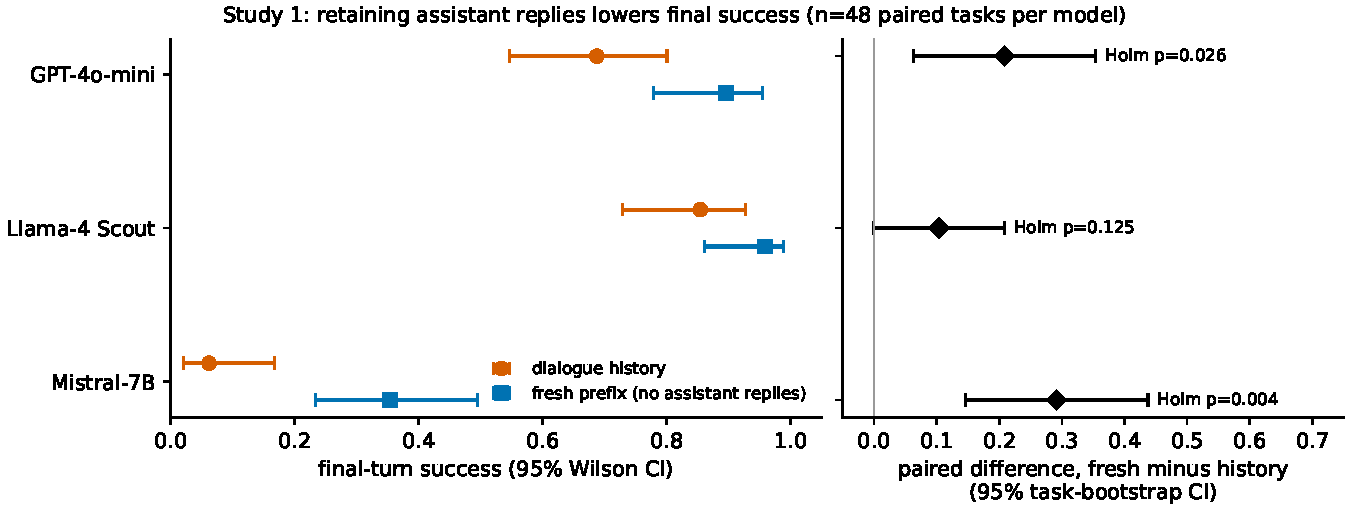
\includegraphics[width=\linewidth]{study1_paired.pdf}
\caption{Study 1 primary endpoint ($n=\nTasks{}$ paired tasks per model).
Left: final-turn success in each arm with 95\% Wilson intervals
\citep{wilson1927probable}. Right: paired difference, fresh prefix minus
dialogue history, with 95\% task-bootstrap intervals and Holm-adjusted McNemar
$p$-values.}
\label{fig:s1}
\end{figure}

\paragraph{The measurable quality metrics do not warn (confirmatory).}
None of CS, LS and SS carried information about final failure beyond turn,
revealed information and context length (Table~\ref{tab:s1rqeval}). All
partial correlations were close to zero, and every Holm-adjusted $p$-value was
1.0. CS had little support, because before the final shard most samples did
not commit to an answer.

\begin{table}[t]
\centering
\caption{Study 1 pre-final metrics as predictors of final failure under
dialogue history. Turns: scored pre-final turns; units: model--task units;
$r_{\text{partial}}$: task-clustered partial correlation; $p$: one-sided
task-clustered permutation test.}
\label{tab:s1rqeval}
\small
\begin{tabular}{lcccccc}
\toprule
Metric & Turns & Units & Tasks & $r_{\text{partial}}$ & $p$ & $p_{\text{Holm}}$\\
\midrule
\inputtable{generated/table_rqeval.tex}
\bottomrule
\end{tabular}
\end{table}

\paragraph{The paired readiness measure reduces to persistence.}
CRL discriminated its frozen target modestly (pooled model-stratified AUROC
\crlAuroc{}, task-clustered permutation $p=\crlP$, bootstrap CI \crlCi{}),
driven by GPT-4o-mini and Mistral-7B (supplementary Table~S2). A post-hoc check
compared CRL with simple baselines. The last pre-final readiness gap alone did
better (AUROC \crlLastGapAuroc{}, $p=\crlLastGapP$), and within strata of that
gap CRL carried no further information (AUROC \crlCondAuroc{},
$p=\crlCondP$). CRL therefore measures the persistence of an unresolved state
rather than anticipating failure beyond the current state. When the target was
replaced, post hoc, by accuracy loss (fresh prefix correct, history wrong), the
association was borderline (AUROC \robAllAuroc{}, $p=\robAllP$) and came from
Mistral-7B alone. Even a paired, counterfactual measure thus did not anticipate
the failure; it registered it once the history arm had already fallen behind.

\section{Study 2: long-horizon degradation under calibrated difficulty}
\label{sec:study2}

\subsection{The CDR-Stream benchmark}

Study 1 tasks span at most nine turns, and their difficulty is not controlled.
To study long horizons, we built CDR-Stream. It consists of 100-turn dialogues
in four domains:
\begin{itemize}
  \item a budget ledger;
  \item inventory logistics;
  \item a laboratory protocol;
  \item milestone chains.
\end{itemize}
Every user turn updates a shared state, for example a delivery, a correction or
a transfer, and asks one question about it. Exact solvers compute the gold
answer of every turn, so accuracy is observable at every turn.

Questions are drawn from six families: sum, difference, count-above-threshold,
maximum, what-if and share. Difficulty follows a 12-level ladder that changes one
complexity axis per step.

\paragraph{Calibrated difficulty.}
Before any stream was generated, a single-turn calibration stage mapped easy,
medium and hard regimes to ladder levels separately for each model and domain.
Its target bands were:
\begin{itemize}
  \item easy: 0.75--0.92;
  \item medium: 0.60--0.78;
  \item hard: 0.35--0.65.
\end{itemize}
The frozen fitting rule used isotonic regression and a one-sided trend test, and
it excluded domains that showed a ceiling, a floor or no trend.
Table~\ref{tab:s2map} lists the resulting mappings.

\paragraph{Scenarios.}
Each regime is a mixture: 50\% of turns at the centre level, 20\% at each
neighbour and 10\% from an adjacent regime. No scenario therefore consists of a
single question type or difficulty. The core scenarios are:
\begin{itemize}
  \item stationary easy (S0-E) and stationary hard (S0-H);
  \item a graded staircase, easy$\to$medium$\to$hard at turns 34 and 68 (S1);
  \item a sudden shift, easy$\to$hard at turn 51 (S2);
  \item a shift with recovery, easy$\to$hard$\to$easy at turns 34 and 67 (S3).
\end{itemize}

\paragraph{Models.}
The models were GPT-4o-mini, Llama-3 70B and Gemma 3 12B. They were chosen
because they passed the calibration rule and a technical pilot, not because of
any stream outcome.

Several other candidates were replaced before the main run:
\begin{itemize}
  \item Mistral-7B was at the accuracy floor;
  \item a larger Gemma model hit the ceiling;
  \item all Llama-4 variants produced near-identical repeated samples.
\end{itemize}
These replacements, and two recorded deviations for Llama-3 70B, are documented
in the supplementary material.

\begin{table}[t]
\centering
\caption{Study 2 frozen difficulty mappings (ladder levels for easy/medium/hard)
by model and domain. A dash marks a domain excluded by the calibration rule.}
\label{tab:s2map}
\small
\begin{tabular}{lcccc}
\toprule
Model & Budget & Inventory & Lab & Chains\\
\midrule
\inputtable{generated/table_cdr_mappings.tex}
\bottomrule
\end{tabular}
\end{table}

\paragraph{Arms and acquisition.}
Each model received 30 held-out dialogues, six per core scenario, each of 100
turns. The two arms were:
\begin{itemize}
  \item \emph{dialogue history}: the model sees all previous user turns and its
    own primary replies, packed into the context;
  \item \emph{verified state summary} (control): the model sees only a
    solver-verified summary of the current state and the current turn.
\end{itemize}
The control arm is a packaged intervention. It shortens the context, removes
noise and supplies correct state, all at once. It therefore tests mitigation,
not mechanism.

The dialogue arm also drew two further samples per turn and two rewordings, so
that consistency, stability and robustness could be measured. All responses
used temperature 0.7 and a 2,048-token ceiling. Responses that reached the
ceiling were kept and scored as missing, under a policy frozen before the main
run.

The analysis protocol was frozen before any main-run metric was computed. The
acquisition paused when the funding budget was exhausted. By then every
dialogue-history primary chain was complete for all three models, together with
all of GPT-4o-mini's samples. The Llama-3 70B and Gemma 3 12B control arms were
subsequently completed under a separately frozen completion protocol; their
primary hypothesis family and missing-data policy were fixed before those data
were inspected.

\subsection{Results}

\paragraph{Accuracy collapses under accumulated history.}
In all three models, dialogue-arm accuracy fell from about 0.6 in the first five
turns to about 0.1 after turn 20 (Table~\ref{tab:s2collapse},
Figure~\ref{fig:s2}). The collapse appeared even in the stationary easy scenario.

Difficulty does not explain it. At the same ladder level, late turns were less
accurate than early turns by \cdrLevelMatched{} on average (prespecified
secondary contrast; $p=\cdrLevelMatchedP$, $n=\cdrLevelMatchedN$ dialogues). In
stationary easy dialogues the difference was \cdrLevelMatchedSzeroE{}.

\begin{table}[t]
\centering
\caption{Study 2 dialogue-arm accuracy (CQ) by turn range, pooled over
scenarios, and in the stationary easy scenario (S0-E). The last column is the
verified-state-summary control over turns 21--100.}
\label{tab:s2collapse}
\small
\begin{tabular}{lccccc}
\toprule
 & \multicolumn{3}{c}{Dialogue history, turns} & S0-E, & State summary,\\
Model & 1--5 & 6--20 & 21--100 & turns 21--100 & turns 21--100\\
\midrule
\inputtable{generated/table_cdr_collapse.tex}
\bottomrule
\end{tabular}
\end{table}

\begin{figure}[t]
\centering
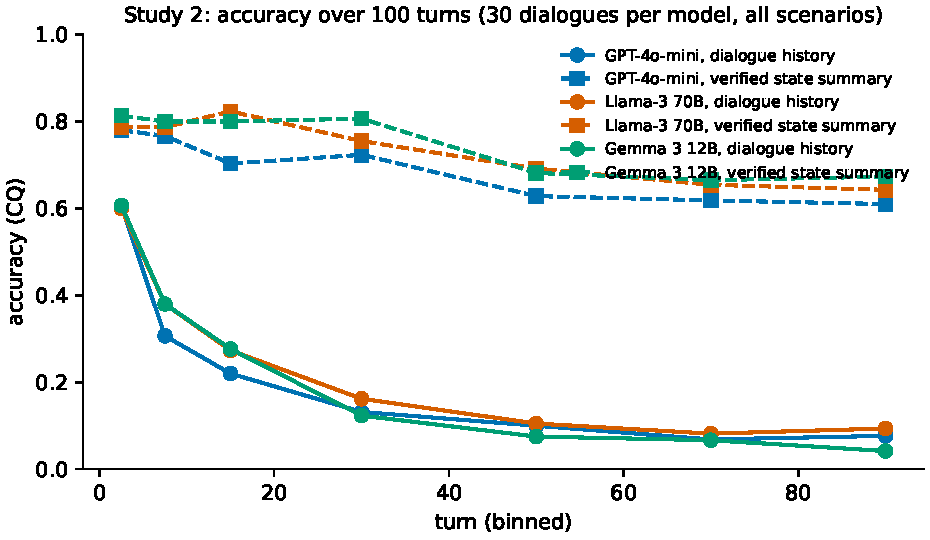
\includegraphics[width=0.85\linewidth]{study2_accuracy_over_turns.pdf}
\caption{Study 2 accuracy over 100 turns, pooled over the five scenarios.
Solid lines show the dialogue history; dashed lines show the verified state
summary. The control's gradual decline reflects the scheduled difficulty
increases in S1--S3.}
\label{fig:s2}
\end{figure}

\paragraph{A verified state summary preserves accuracy.}
GPT-4o-mini answered the same questions from the verified state summary with an
accuracy of \cdrGptCtrlLate{} over turns 21--100, against \cdrGptLate{} under
dialogue history. Under the summary its accuracy also followed the scheduled
difficulty regimes.

The frozen completion test confirmed this mitigation in the two-model family.
Over turns 1--100, the per-dialogue control-minus-history gap was
\cdrLlamaControlGap{} for Llama-3 70B (95\% bootstrap CI
[\cdrLlamaControlCiLo{}, \cdrLlamaControlCiHi{}]) and
\cdrGemmaControlGap{} for Gemma 3 12B (95\% CI
[\cdrGemmaControlCiLo{}, \cdrGemmaControlCiHi{}]); both one-sided sign-flip
tests remained significant after Holm correction
($p=\cdrLlamaControlHolmP{}$ and $p=\cdrGemmaControlHolmP{}$, respectively;
30 paired dialogues per model). The secondary turns 21--100 gaps were
\cdrLlamaControlLateGap{} and \cdrGemmaControlLateGap{}. Table~\ref{tab:s2control}
reports the frozen primary family, including the previously observed
GPT-4o-mini estimate outside that family.

\begin{table}[t]
\centering
\caption{Frozen H-C1: per-dialogue mean accuracy difference between verified
state summary and dialogue history over turns 1--100. The GPT-4o-mini result
was already observed and was excluded from the Holm family.}
\label{tab:s2control}
\small
\begin{tabular}{lcccc}
\toprule
Model & Mean gap & 95\% bootstrap CI & Holm $p$ & Dialogues\\
\midrule
\inputtable{generated/table_cdr_control_completion.tex}
\bottomrule
\end{tabular}
\end{table}

Because the dialogue arm was already near the floor, the frozen pre/post
change-point contrasts of the dialogue arm were dominated by the background
collapse. We therefore do not interpret them as task-drift effects (see the
supplement).

\section{Can the degradation be detected early?}
\label{sec:monitoring}

Both studies show that accumulated history can lower accuracy substantially. A
deployed expert system, however, does not observe accuracy. We therefore asked
whether the monitoring framework of Section~\ref{sec:framework} would have
warned. We asked at three levels: the direction of the individual quality
metrics, the alarms of calibrated single-stream detectors, and the statistical
power that such detectors can have at all. Table~\ref{tab:warningsummary}
summarises the answers; none yielded robust, model-general early warning.

\begin{table}[t]
\centering
\caption{Summary of the early-warning tests. Labels follow
Section~\ref{sec:framework}.}
\label{tab:warningsummary}
\small
\resizebox{\linewidth}{!}{\begin{tabular}{p{0.20\linewidth}p{0.25\linewidth}p{0.13\linewidth}p{0.32\linewidth}}
\toprule
Setting & Signal & Label & Outcome\\
\midrule
Study 1, pre-final turns & CS, LS, SS vs.\ final failure & confirmatory &
no association; all Holm $p=1.0$\\
Study 1 & CRL (paired readiness) & confirmatory, auxiliary & modest AUROC
\crlAuroc{}; no information beyond last readiness gap (post hoc)\\
Study 1 replay & five detectors on CQ, CS, RS, LS, SS & post hoc &
detection $\le0.067$ under family-wise control; no candidate\\
Study 2, history arm & six metrics, three strategies & confirmatory &
CQ nulls also collapse, so thresholds cannot be calibrated; other metrics
$\le0.11$\\
Study 2, GPT control & CQ, LS, ES detectors and threshold rule & exploratory
& CUSUM \ctrlScreenDetect{}; LS leads not separable from null alarms\\
Study 2, Llama/Gemma control & unchanged rules & confirmatory validation &
screen failed in both models\\
Study 2, six-dialogue aggregates & CQ CUSUM & exploratory & all drift
scenarios detected; one stationary alarm (Gemma)\\
\bottomrule
\end{tabular}}
\end{table}

\subsection{Quality metrics do not fall with accuracy}

In Study~1, the pre-final CS, LS and SS carried no information about final
failure (Table~\ref{tab:s1rqeval}). A post-hoc stream replay shows why
(Figure~\ref{fig:silent}b). Completed Study~1 sessions were treated as stream
items whose regime switched from fresh prefix to dialogue history. Coherence and
stability \emph{rose} after the switch while accuracy fell. In the sudden
scenario at $W=20$, the median Cliff's $\delta$ \citep{cliff1993dominance}
between the last pre-change and post-change windows was \replaySsDeltaGpt{}
for SS in GPT-4o-mini and \replaySsDeltaLlama{} in Llama-4 Scout, and
\replayLsDeltaGpt{} for LS in GPT-4o-mini.

Study~2 shows the same pattern over 100 turns (Figure~\ref{fig:silent}a). This
part is descriptive. For GPT-4o-mini under dialogue history, accuracy fell from
\silentCQEarly{} in turns 1--5 to \silentCQLate{} in turns 81--100. Over the
same span, trace stability rose from \silentSSEarly{} to \silentSSLate{} and
logical coherence moved only from \silentLSEarly{} to \silentLSLate{}.
Answer consistency declined from \silentCSEarly{} to \silentCSLate{}, but
slowly and long after most of the accuracy had been lost. It even rose over turns
6--15, when accuracy halved. As the model fails, its replies become more
mutually similar and stay locally coherent. A monitor that alarms on
\emph{decreases} of these metrics cannot detect this pattern by construction,
and a two-sided monitor would detect a change whose sign carries no reliable
meaning about correctness.

\begin{figure}[t]
\centering
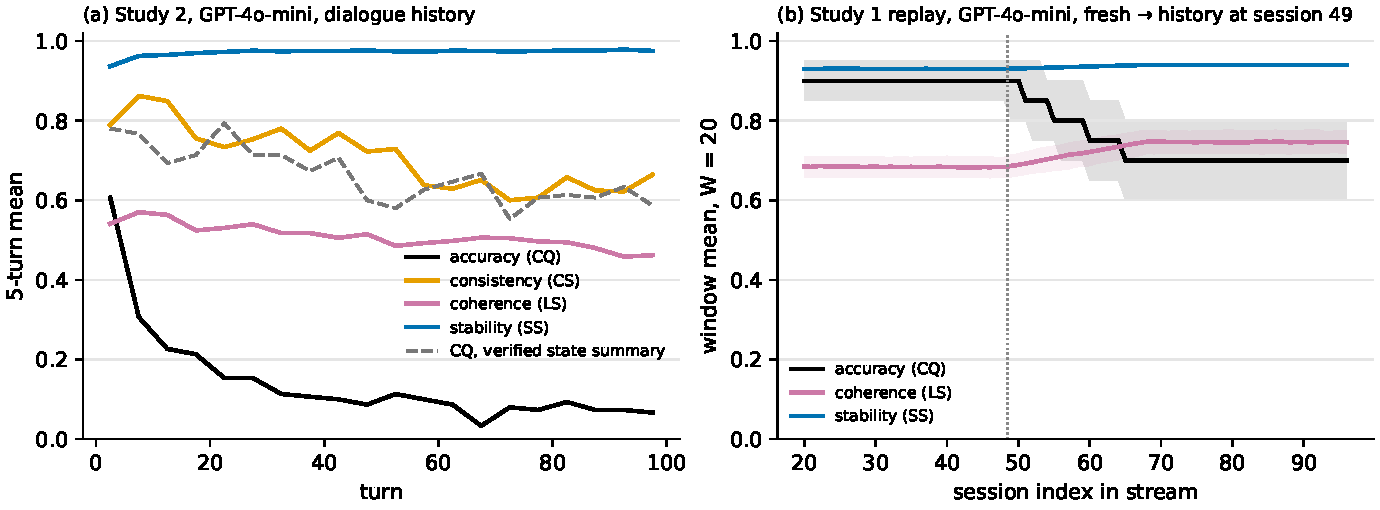
\includegraphics[width=\linewidth]{silent_metrics.pdf}
\caption{Quality metrics do not track accuracy. (a) Study 2, GPT-4o-mini,
dialogue history, means over 5-turn bins across 30 dialogues (descriptive);
the dashed line is accuracy under the verified state summary. CS is supported
by \silentCsSupport{} of 3,000 turns. (b) Post-hoc replay of Study 1 sessions:
median and 10--90\% band over 1,000 orderings of window means ($W=20$) when the
regime switches from fresh prefix to dialogue history at session 49.}
\label{fig:silent}
\end{figure}

\subsection{Calibrated single-stream detectors}

\paragraph{Study 1 replay (post hoc).}
In the replay, thresholds were calibrated on 2,000 permutation nulls with
family-wise $\alpha=0.05$ and validated on 2,000 disjoint nulls. Under that
control, the best detection rate for any metric, detector and strategy was
0.067 (Mistral-7B, CQ, sudden switch), with a median delay of about 44
sessions. No metric qualified as an early-warning candidate
(supplementary Table~S4).

\paragraph{Study 2, dialogue-history arm (confirmatory).}
The stationary dialogues that should serve as nulls themselves collapsed. For
CQ no grid value kept the null false-alarm rate at 5\% in most configurations,
so a threshold could not be calibrated at all. For the other metrics, detection
within 33 turns of the first change was at most 0.11. This is the core
difficulty of monitoring under accumulated history. The context-driven decline
starts at turn~1, before any detector has a reference period, and it is
present in exactly the streams that define normal behaviour.

\paragraph{Study 2, verified-state arm (exploratory, then validated).}
The control arm removes the background collapse and leaves only the scheduled
task drift, which makes it the cleanest test of the detectors themselves. On
GPT-4o-mini, with thresholds calibrated on the 12 stationary dialogues, CUSUM on
the window mean of CQ detected \ctrlScreenDetect{} drift dialogues within 33
turns at $W=20$. One reason is structural: the detectors ignore their first 20
window values, so at $W=20$ the earliest alarm falls near turn 40, after the
first change at turn 34. A simpler per-dialogue rule signals when the window
mean falls below $\mu_0-2\sigma_0/\sqrt{W}$ on three consecutive turns, with
$\mu_0$ and $\sigma_0$ taken from turns 1--30. It flagged accuracy in
\earlyCqSignal{} drift dialogues but also in \earlyCqNull{} stationary ones. LS
signalled in \earlyLsSignal{} drift dialogues, \earlyLsBefore{} of them before
accuracy, but also in \earlyLsNull{} stationary dialogues. Its apparent lead is
therefore not separable from noise.

These rules had been fixed after GPT-4o-mini trajectories were seen, so we
applied them unchanged to the unseen Llama-3 70B and Gemma 3 12B control arms
as a frozen validation. CUSUM detected \valLlamaDetect{} Llama drift dialogues
(median delay \valLlamaDelay{} turns) and \valGemmaDetect{} Gemma dialogues
(delay \valGemmaDelay{}), and neither model passed the frozen screen. The LS
rule signalled in \valLlamaLsSignal{} and \valGemmaLsSignal{} drift dialogues,
but also in \valLlamaLsNull{} and \valGemmaLsNull{} stationary dialogues. The
validation confirms that neither rule gives robust, model-general early
warning.

\subsection{Why single streams are underpowered}

The detector failures are not specific to our metrics. They follow from the
amount of information in one 100-turn stream. We simulated per-turn
correctness streams with pre-change accuracy 0.80 and a drop $\delta$ at turn
34 or 51. Each simulated turn aggregated $m$ independent dialogues. We used the
unchanged detectors and grids, calibrated thresholds on 12 null streams at a
5\% false-alarm target, and drew 300 drift streams per cell
(Table~\ref{tab:power}, Figure~\ref{fig:power}). A single stream reached 80\%
detection within 33 turns only for drops of about 0.5. The task drifts in our
data were 0.1--0.3. Aggregating six concurrent dialogues per turn brought the
detectable drop to 0.2, and 18 dialogues brought it to 0.1. Results were
similar for $W=10$ and $W=30$ and for larger calibration sets (supplement).

\begin{table}[t]
\centering
\caption{Simulated detector power: best unchanged detector, $W=20$, thresholds
from 12 null streams, 5\% false-alarm target. Columns 2--3: smallest accuracy
drop detected within 33 turns in at least 80\% of runs. Column 4: detection
rate for a drop of 0.2, averaged over both change points.}
\label{tab:power}
\small
\begin{tabular}{cccc}
\toprule
Dialogues per turn & Change at 34 & Change at 51 & Detection at $\delta=0.2$\\
\midrule
\inputtable{generated/table_power.tex}
\bottomrule
\end{tabular}
\end{table}

\begin{figure}[t]
\centering
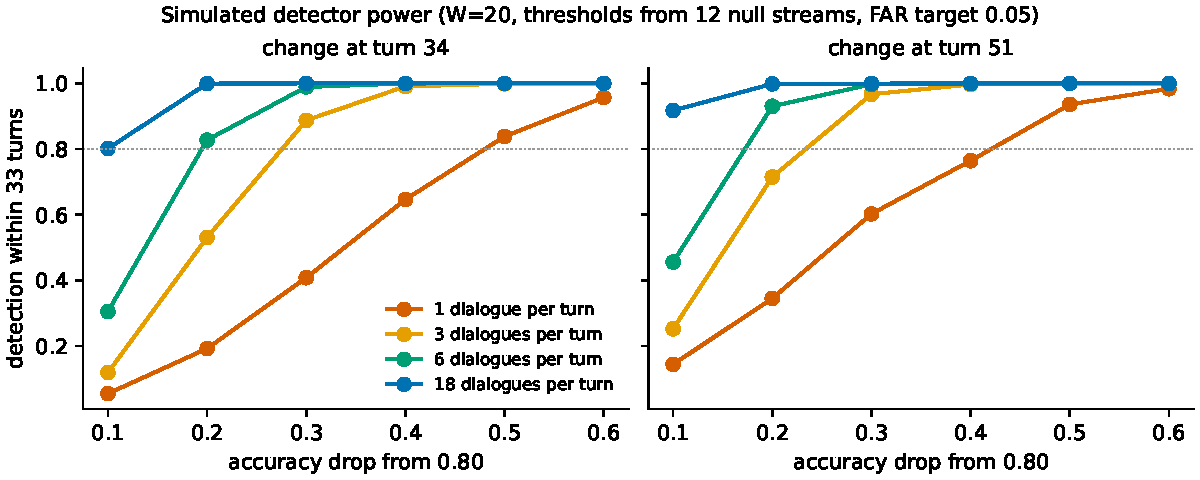
\includegraphics[width=\linewidth]{detector_power.pdf}
\caption{Simulated detection within 33 turns as a function of the accuracy drop
from 0.80 and the number of dialogues aggregated per turn ($W=20$, thresholds
from 12 null streams, 5\% false-alarm target). Left: change at turn 34; right:
change at turn 51. The dotted line marks 80\% detection.}
\label{fig:power}
\end{figure}

We then applied this idea to the control arms, which is exploratory. A CQ
CUSUM on the mean of the six dialogues of each scenario, with $W=20$, detected
all three drift scenarios in both validation models (\valLlamaAggDetect{} and
\valGemmaAggDetect{}). It raised no alarm in the two Llama stationary
aggregates but one in the two Gemma stationary aggregates (\valLlamaAggNull{}
and \valGemmaAggNull{}). Together with the GPT-4o-mini screen, this supports
aggregation across sessions as a promising direction. The small number of
scenario-level aggregates and the Gemma false alarm, however, preclude a
confirmatory claim.

\subsection{A baseline that could not fire}

In our generic ADWIN-everywhere baseline, ADWIN never alarmed in any analysis.
The cause was in our implementation. Its cut bound omitted the variance term of
\citet{bifet2007learning}, and without that term no difference of means in a
stream of at most 100 values in $[0,1]$ can exceed the bound. We re-ran every
affected analysis with a corrected ADWIN and with CUSUM in its place, as a
labelled sensitivity analysis. No conclusion changed: consistency and stability
still did not give early warning, so their earlier ``no warning'' result is now
genuinely tested rather than an artefact. Even the corrected ADWIN needed drops
of about 0.6 to detect reliably on 100-turn streams (supplement). The lesson is
general: a comparison against a generic baseline is only meaningful once the
baseline has been shown to fire on streams of the intended length.

\section{Discussion}
\label{sec:discussion}

\paragraph{Two complementary failure modes.}
The two studies reveal two complementary ways in which multi-turn context can
degrade reasoning.

\begin{itemize}
  \item \textbf{Short tasks (Study 1).} Retaining the assistant's own replies
    lowered final success relative to an information-matched context without
    them. This replicates the direction reported by \citet{huang2026benefit}
    under a frozen, task-paired analysis. Mistral-7B illustrates one mechanism:
    with its own replies in context it tended to remain in an explicit ``need
    more information'' state, while the same model given the same information
    without those replies attempted an answer.
  \item \textbf{Long horizons (Study 2).} With a steadily updated state, accuracy
    collapsed within about twenty turns, even at fixed difficulty. A verified
    state summary avoided the collapse \pending{in all three models}.
\end{itemize}

The studies differ in tasks, models and controls. We therefore do not claim that
the short-task effect causally grows into the long-horizon collapse. Study 2 also
cannot separate three possible causes: history length, the number of state
updates, and error accumulation.

\paragraph{Why quality metrics stay silent.}
Consistency, coherence and stability measure local properties of responses. A
model that has committed to a wrong premise or a wrong state can reason
coherently and repeatably from it. In our replay these metrics even rose as
accuracy fell, which suggests that accumulated context makes responses more
anchored.

The paired process measure fared no better than the current readiness state
itself. Accuracy-based detectors, for their part, are limited by the noise of a
single stream. Monitoring designs that assume quality metrics fall before
accuracy are therefore unlikely to work in this setting. Token-level uncertainty
signals such as those used by ERGO \citep{khalid2025ergo} are a different class
of signal. We did not test them, because our protocols did not collect token
probabilities.

\paragraph{Implications for practice.}
Three practices follow from our results:
\begin{itemize}
  \item Do not let the raw history grow indefinitely in tasks that maintain
    state. Re-ground the model periodically in a compact, verified state
    representation.
  \item Monitor by comparison: against a verified-state or history-free
    re-query, or across many concurrent sessions. Single-stream quality
    trajectories are not a substitute.
  \item Before using a generic drift detector as a comparator, verify that it
    can fire on streams of the intended length.
\end{itemize}

\paragraph{Limitations.}
\begin{itemize}
  \item \textbf{Scope.} Both studies use arithmetic reasoning with exact answers
    and models available through one academic gateway, and the two studies use
    different models. Effects may differ for other domains, newer models or other
    serving stacks.
  \item \textbf{Net effects.} Study 1 estimates the net effect of retaining
    assistant replies, which contain both harmful commitments and potentially
    useful work. Study 2's control is a packaged intervention, not a mechanism
    test.
  \item \textbf{Observability.} Accuracy, robustness and efficiency were
    unobservable before the final turn in Study 1. Their early-warning value
    there was not tested.
  \item \textbf{Exploratory analyses.} The Study 2 monitoring analyses, the CRL
    persistence check, the accuracy-loss target and the stream replay are
    exploratory or post-hoc, and are labelled as such.
  \item \textbf{Study 2 acquisition.} A funding pause staged the acquisition.
    \pending{The frozen completion of the control arm, and the status of the
    remaining consistency, robustness and stability samples, which are reported
    for GPT-4o-mini only.}
  \item \textbf{Single investigator.} The audit of Study 1 tasks and the
    calibration of Study 2 were carried out by one investigator.
\end{itemize}

\section{Conclusion}
\label{sec:conclusion}

Across two frozen studies, retaining assistant history reduced short-task
success, and accumulated history caused a rapid 100-turn collapse that verified
state prevented in all three tested models. No examined quality metric, paired
process measure or single-stream detector provided robust model-general warning.
Reliable long interactions therefore require explicit state management and,
where monitoring is needed, comparative or aggregated evidence rather than a
single apparently coherent trajectory.


\section*{Data and code availability}
All prompts, frozen protocols, configurations, analysis code and the scripts
that generate every number, table and figure in this article are maintained in
a version-controlled
\href{https://github.com/senolali/reasoning-monitor-3501}{GitHub repository}.
The repository is private during manuscript preparation. A public archival
release with a persistent DOI, derived data and provider-permitted model
responses will be made no later than publication.

\section*{Acknowledgements}
This work was supported by the Scientific and Technological Research Council of
T\"urkiye (T\"UB\.{I}TAK) under the 3501 programme, project number 126E663.
Model inference was performed through Arizona State University's CreateAI
research infrastructure.

\section*{Declaration of competing interest}
The author declares that he has no known competing financial interests or
personal relationships that could have appeared to influence the work reported
in this paper.

\section*{CRediT authorship contribution statement}
Ali \c{S}enol: Conceptualization, Methodology, Software, Validation, Formal
analysis, Investigation, Data curation, Visualization, Writing--original draft,
Writing--review and editing, Project administration, Funding acquisition.

\bibliographystyle{elsarticle-harv}
\bibliography{references}

\end{document}
